%!TEX TS-program = xelatex
%!TEX encoding = UTF-8 Unicode

\documentclass[11pt]{article}
\usepackage{geometry}            % See geometry.pdf to learn the layout options. There are lots.
\geometry{a4paper}                   % ... or a4paper or a5paper or ... 
%\geometry{landscape}                % Activate for for rotated page geometry
\usepackage[parfill]{parskip}    % Activate to begin paragraphs with an empty line rather than an indent
\usepackage{graphicx}
\usepackage{amssymb}
\usepackage{lipsum}
\usepackage{multicol}
\usepackage{lettrine}
\usepackage[italian]{babel}
\usepackage{fancyhdr}
\usepackage{hyperref}
\usepackage{musicography}
%\usepackage{quote}



\usepackage{fontspec,xltxtra,xunicode}
\defaultfontfeatures{Mapping=tex-text}
\setromanfont[Mapping=tex-text]{Palatino}
\setsansfont[Scale=MatchLowercase,Mapping=tex-text]{Avenir Next Condensed}
\setmonofont[Scale=MatchLowercase]{Andale Mono}

 
\pagestyle{fancy}
%\fancyhf{}
\rhead{\textsf{TEMPLATE XXX -  2020/04/13}}
%\lhead{Guides and tutorials}
\cfoot{\thepage}
\renewcommand{\headrulewidth}{5pt}
\renewcommand{\footrulewidth}{1pt}
 
 \begin{document}
\begin{minipage}{0.55\linewidth}
\vspace{0.3cm}
{\large{\textbf{\textsf{Galileo Galilei}}}}\\
{\normalfont Mstematico Sopraordinario\\
dello Stvdio di Pisa\\
Pisa (PI)\\
{\textsf{\emph{email[at]domine[dot]xxx}}}}
\end{minipage}
\quad
\begin{minipage}{0.42\linewidth}
\begin{flushright}

{\huge{\textbf{\textsf{Lesson I}}}} \\
{\LARGE{\textbf{{\textsf{Dialogo\\ Sopra i Due\\ Massimi Sistemi
}}}}}\\
\end{flushright}
\end{minipage}
\vspace*{0.3cm}

%=========ABSTRACT===============================

\textsf{\textbf{
			\lipsum[1]
		}}


%=========FOREWORD========================

\begin{multicols*}{2}
\lettrine {A}{e} 
			\lipsum[1]


%=========FIRST=============================


\textbf{\textsf {First}}

\lipsum[1]


\begin{center}
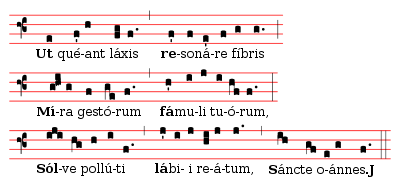
\includegraphics[scale=0.5]{images/utque.png}
{\scriptsize \emph{fig.1 }}
\end{center}

\lipsum[2]

%=========SECOND=================================



\textbf{\textsf {Second}}

\lettrine {A}{e} \lipsum[1]

\begin {quote}
\emph{ \lipsum[1] }


\end{quote}

Abc\footnote{\textbf{\textsf {\lipsum[1]}}}
\lipsum[2]




\vfill
\columnbreak

%===============================================

\textbf{\textsf {Biblio}}\\
•\textsc{\textsf {Name Surname}}, \emph{Title}, Editor 1990\\
•\textsc{\textsf {Name Surname}}, \emph{Title}, Editor 2000\\




















\end{multicols*}

\end{document}  